\chapter{Preprocesado de datos}


Una vez examinados todos los conjuntos mencionados anteriormente, podemos llevar a cabo la unión de todos los datos en un único subconjunto. Esto nos permitirá conseguir un dataset completo y variado con diferentes tipos de piel y diferentes lesiones que nos permitirán identificar multitud de tipos de patologías, siendo posible ajustar el grado de granularidad en función de la agrupación o no de posibles subclases.

Inicialmente, el conjunto de datos construido contendrá todos los subtipos de lesiones cutáneas vistos, pero dispondrán de una segunda etiqueta que indicará si se trata de un caso canceroso o no, atendiendo a su subclase que lo etiqueta. Si agrupamos por lesiones benignas, cancerosas, y potencialmente cancerosas, podemos obtener el siguiente diagrama de sectores de la figura \ref{tartabinaria}, donde se puede observar cómo la mayoría de imágenes disponibles engloban problemas de piel no cancerosos, mientras que el segundo tipo más común de lesión si es la cancerosa. Si atendemos a clasificar las subclases de cada tipo de patología, encontramos 52 posibles etiquetas, las cuales iremos examinando a medida que se preprocese cada uno de los subconjuntos.


\begin{figure}[H]
	\centering
	\label {tartabinaria}
	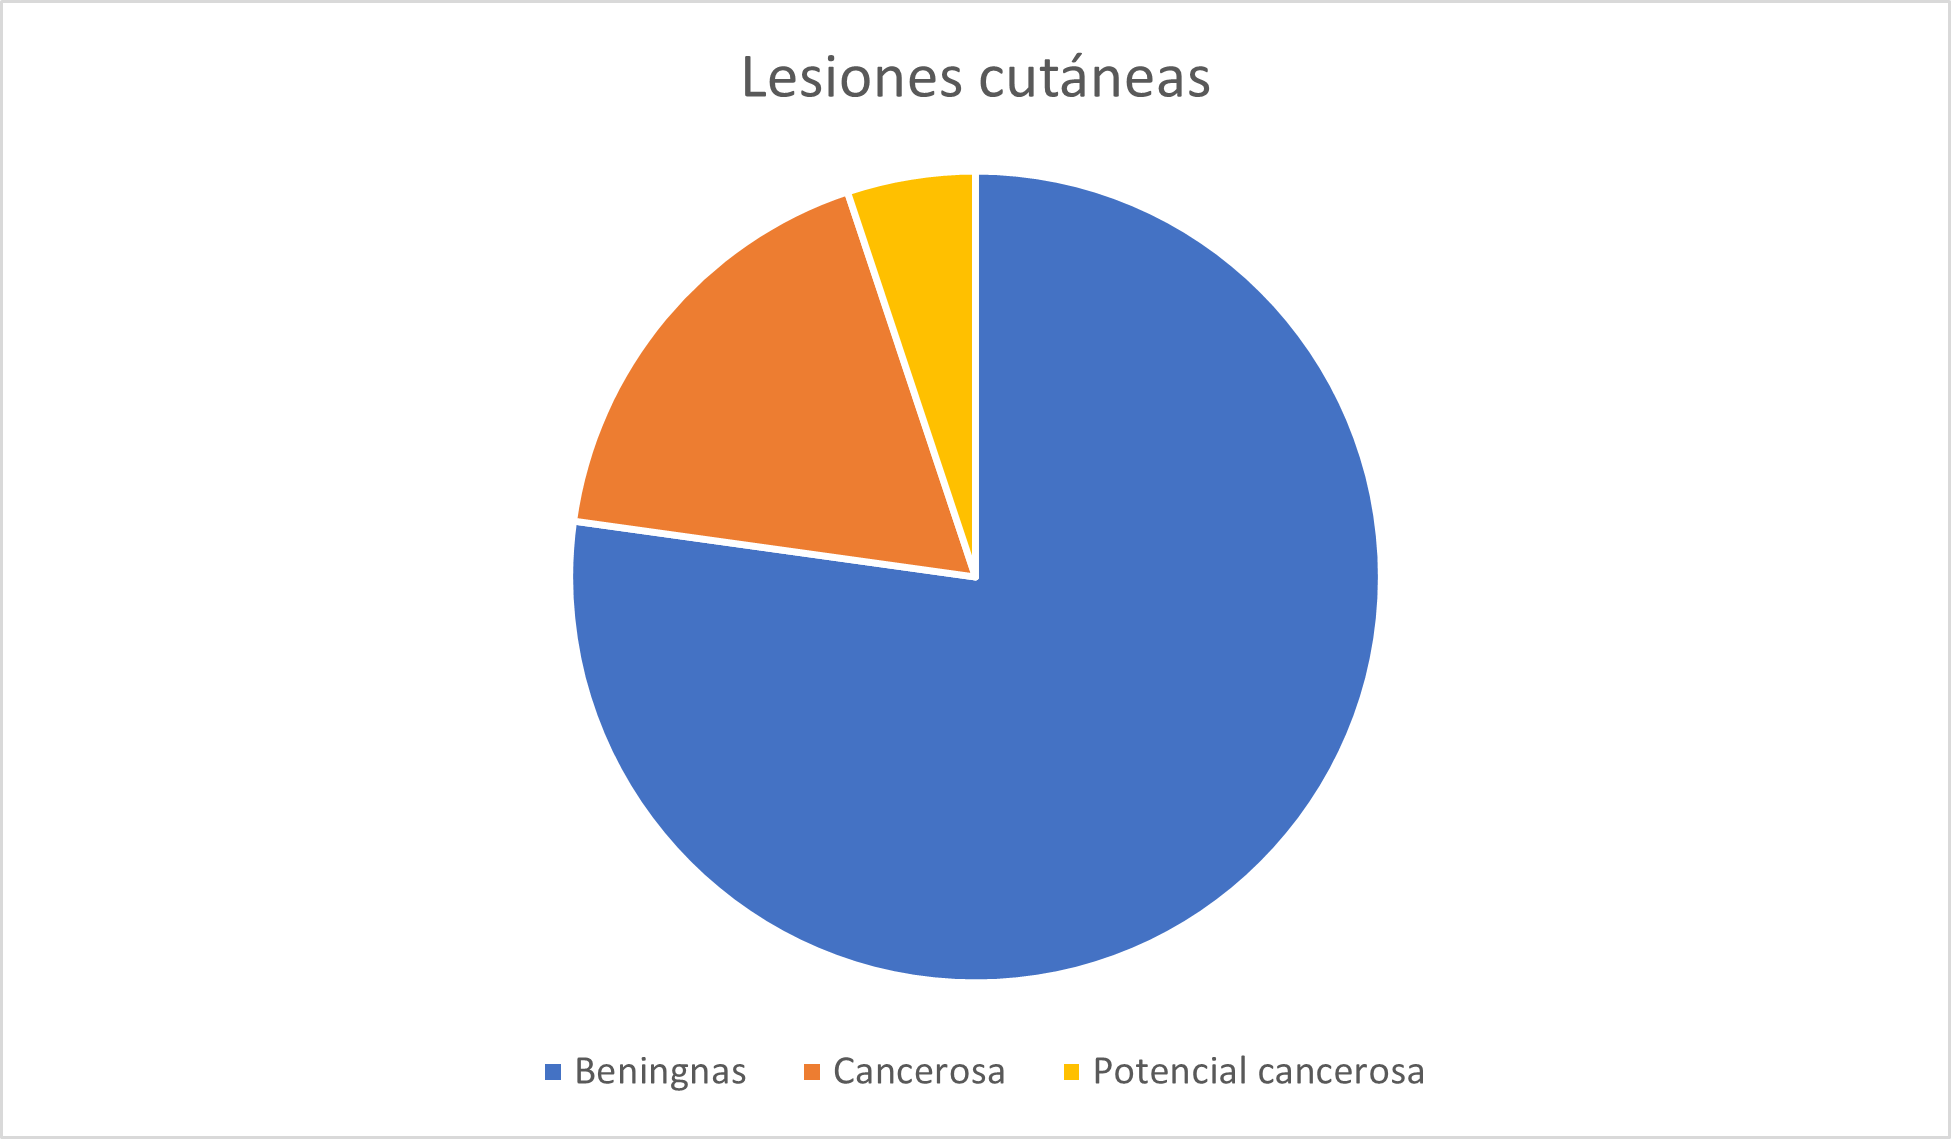
\includegraphics[scale = 0.7]{imagenes/datasetfinal.png}
	\caption{Distribución de clases}
\end{figure}

En el caso de las lesiones potencialmente cancerosas, como se trata de condiciones de la piel no cancerosas con posible evolución a cancerosas, se tendrán en cuenta como imágenes benignas, ya que la condición de malignidad sólo podría aparecer en el futuro, el cual sigue siendo desconocido.

El preprocesado de datos es una fase indispensable para el correcto aprendizaje de los algoritmos de deep learning. Se ha demostrado empíricamente que una correcta preparación y normalización de los datos permiten hallar soluciones más cercanas a la optima que con datos no procesados.

Es importante tener en cuenta que no existe una metodología de preprocesado única, y que es necesario adaptarse al tipo de dato que estamos tratando. Para este proyecto, además, existe una dificultad adicional, y es la existencia de diferentes procedencias para los datos, pues en total se dispone de 5 datasets distintos, cada uno recopilado con diferentes metodologías e instrumentación. Por tanto, será clave adaptarse a cada uno de los destinos, y realizar la partición final de forma estratificada para evitar sesgos que perturben el resutado.

a continuación, se describe la estrategia seguida para el procesado global de los datos, y los ajustes necesarios para cada uno de los conjuntos empleados.

\section{Estrategia de preprocesado para la fusión}

En el punto de partida, antes del preprocesado, contamos con 5 datasets muy diferentes entre sí. Cada uno ha sido documentado y organizado siguiendo unos criterios no estándares que nos afectan en gran medida a la hora de emplear estos datos para el aprendizaje. Antes de proceder con el desarrollo de los modelos, debemos de estadarizarlos a un formato común para evitar que existan clases con el mismo diagnóstico que, por cuestiones de formato, se consideren etiquetadas como clases distintas, por usar criterios distintos de escritura, como ausencia de espacio, mayúsculas o one hot encoding. 

Concretamente, los datos recopilados poseen el siguiente formato de etiquetado:
\begin{itemize}
	\item ISIC: etiquetas escritas a formato completo, como nombre de carpeta, con la primera letra de la enfermedad en mayúscula.
	\item ASAN: nombres escritos en el nombre de la fotografía, haciendo uso de caracteres especiales, y de abreviaturas.
	\item Severance: etiquetas escritas en la propia imagen, la cuales habrá que etiquetar y organizar manualmente, debido a que su csv está incompleto.
	\item PH2: fichero csv, con diagnósticos en formato one hot encoding. Es decir, una fila de ceros y unos, siendo uno la clase a la que pertenece, y 0, el resto.
	\item PAD UFES 20: fichero csv, con los nombres de diagnóstico escritos en minúsculas, sin espacios.
\end{itemize}

Podemos observar la gran variedad de formatos de registro empleados, y que por tanto, es completamente obligatorio y necesario realizar una transformación para hacerlo homogéneo. En este caso, por decisión propia, he considerado adecuado realizar una transformación de las etiquetas al siguiente formato: Uso únicamente de minúsculas, con ausencia de caracteres especiales, nombres sin abreviaturas, y evitando el uso de espacios, con el uso de la barra baja como carácter sustitutivo. Para la clasificación binaria, se utilizará one hot encoding, denotando como 0 los casos negativos y como unos, los positivos.\\


De esta forma, se obtiene un fichero .csv donde encontrar los valores necesarios para entrenar los modelos. Para poder localizar cada imagen, se mantendrá el arbol de directorios por defecto de cada dataset, y se anotará su directorio en un nuevo fichero .csv, que contendrá las etiquetas estandarizadas y los nombres de los ficheros de imagen con y sin el directorio. En resumen, contará con los campos:

\begin{itemize}
	\item image: nombre la imagen, sin el path en su nombre, y con la extensión de formato
	\item dir: directorio donde se aloja la imagen, respetando la estructura de carpetas original seguida por el dataset de origen
	\item label: etiqueta con el diagnóstico de la lesión, siguiendo las pautas indicadas anteriormente
	\item dataset: columna que indica el dataset de procedencia de la imagen, por si fuese necesario utilizar solo un subconjunto de todos los datos.
	\item bin: columna para la etiqueta que indica si se trata de clase Benigna (0) o Maligna (1)
\end{itemize}

\begin{figure}[H]
	\centering
	\label {formatocsv}
	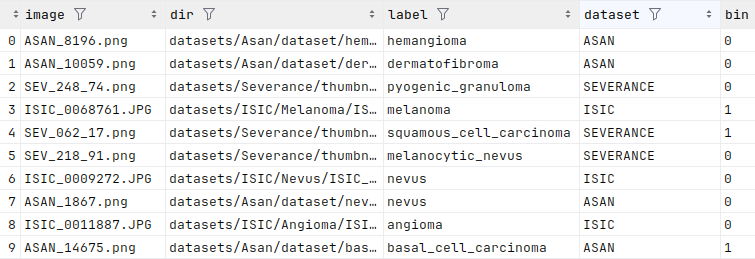
\includegraphics[scale = 0.55]{imagenes/formatocsv.png}
	\caption{Formato del fichero csv normalizado}
\end{figure}

Una vez establecido el formato común, podemos pasar al análisis y adaptación propia de cada conjunto.

\subsection{ISIC Dataset}





